\part{Evaluation}
\label{part:evaluation}


%------------------------------------
\section{Internal evaluation of the GAN}
\label{sec:internal_validation}

\begin{wrapfigure}{r}{0.4\textwidth}
    \centering
    \vspace*{-20pt}
    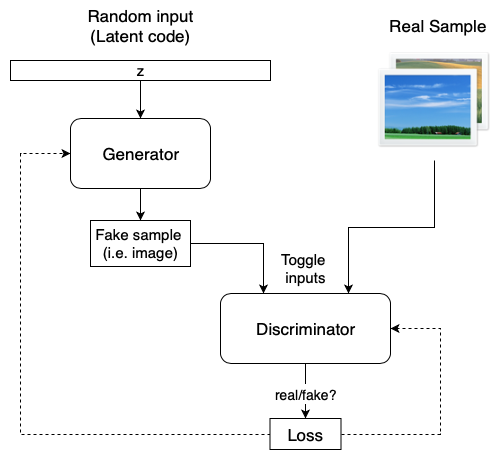
\includegraphics[width=0.35\textwidth]{images/howganwork.png}
    \captionsetup{justification=centering}
    \caption{Illustration on how a GAN works by \citet{how_gan_works}.}
    \label{fig:howganworks}
\end{wrapfigure}

Validation is already a crucial component in the working of a GAN.
A GAN works by training 2 individual AIs, a generator and a discriminator.
The former generates images from scratch.
The discriminator then tries to validate whether the image generated by the generator is real or not.
The training images are thus for the learning algorithm of the discriminator.
The output of the discriminator is then used as a way of validating and evaluating the output of the generator and training it further.
It is clear this process forms a sort of cat and mouse game between both AIs, an analogy often made when talking about GANs.
A visual of this is given in figure \ref{fig:howganworks}, taken from an easy explanation on how StyleGAN works by \citet{how_gan_works}.

So in a way, a GAN is internally evaluated by design.
ProGAN, in many ways a precursor to StyleGAN, also from NVIDIA, was exceptional in the way it works by having a discriminator and generator whose performance increases over time.
This happens by incrementally increasing the resolution, expressed in the number of pixels, of both models.
This idea is still in place with StyleGAN, which again proves a form of internal, increasingly harder, evaluation plays a key role in its working.

%------------------------------------
\section{Building the external evaluation tool}
\label{sec:evaluation_tool}

Since internal evaluation is already taken care of by design, the focus of this project lies in external evaluation.
Besides using the criteria and framework seen in the course, a survey with juries will also be held.
For this survey, a custom PHP tool was developed by modifying a tool used in a previous paper \citep{bapproef} of mine.
A screenshot of the tool is given in figure \ref{fig:eval_tool}.
The flow of this custom made tool is as follows:
\begin{itemize}
    \item Explain what data of the participant will be stored and made available to the public.
    \item Show a short video explaining the different criteria the participant will have to fill out for each image.
    \item Ask personal info about participant:
    \begin{itemize}
        \item Gender, since some car designs might appeal more to a certain gender.
        \item Age group, separated in 5-year intervals to further anomalies the participant info. 
        \item Whether or not the participant has expertise in the domain. A participant is considered to have expertise in the domain if he can recognize cars from different brands from any angle, albeit since he is a passionate car lover or works in a garage or anything in between.
        \item Whether or not the participant is colour blind or has restricted vision during the survey.
    \end{itemize}
    \item Show some 'test images' first that can be used to tackle burn-in of the rating system.
    \item Show images one by one in random order and ask the participant the following using a likert scale from zero to five:
    \begin{itemize}
        \item Quality: an image is considered of good quality if it doesn't contain graphical glitches or artefacts as explained in the introductory video.
        \item Colors: colours of an image are considered good if they are viable in real life. Remember, some colour combinations may be ugly to the participant but still realistic. An image has bad colours if it has purple grass, red shadows...
        \item Creativity: whether the participant finds the image creative is a subjective manner, if the participant recognize (elements of) existing cars (s)he can discuss this in the notes field.
        \item General impression: an overall rating on how pleased the participant is with this car design. This is again subjective with possible further discussion in the notes.
        \item Notes: this field can be used to discuss recognised cars, the reasoning for exceptionally low or high scores and more.
    \end{itemize}
\end{itemize}

%------------------------------------
\section{Further notes on evaluation}
\label{sec:notes_evaluation}

The evaluation criteria are still open for debate.
Initially, the user is told he will see images of both human-made car design through Adobe Photoshop and computer-generated car design.
Whether or not the user is shown an image as human-made or machine-generated is at random and stored in the database.
This was done to combat bias but is again still open for changes.
The tool is already published online \footnote{\url{https://car-design-survey.lennertbontinck.com/}} for feedback purposes of this assignment. 
Note that the introductory video explaining the tool is not yet made and thus not yet available. 

\begin{figure}[H]
    \centering
    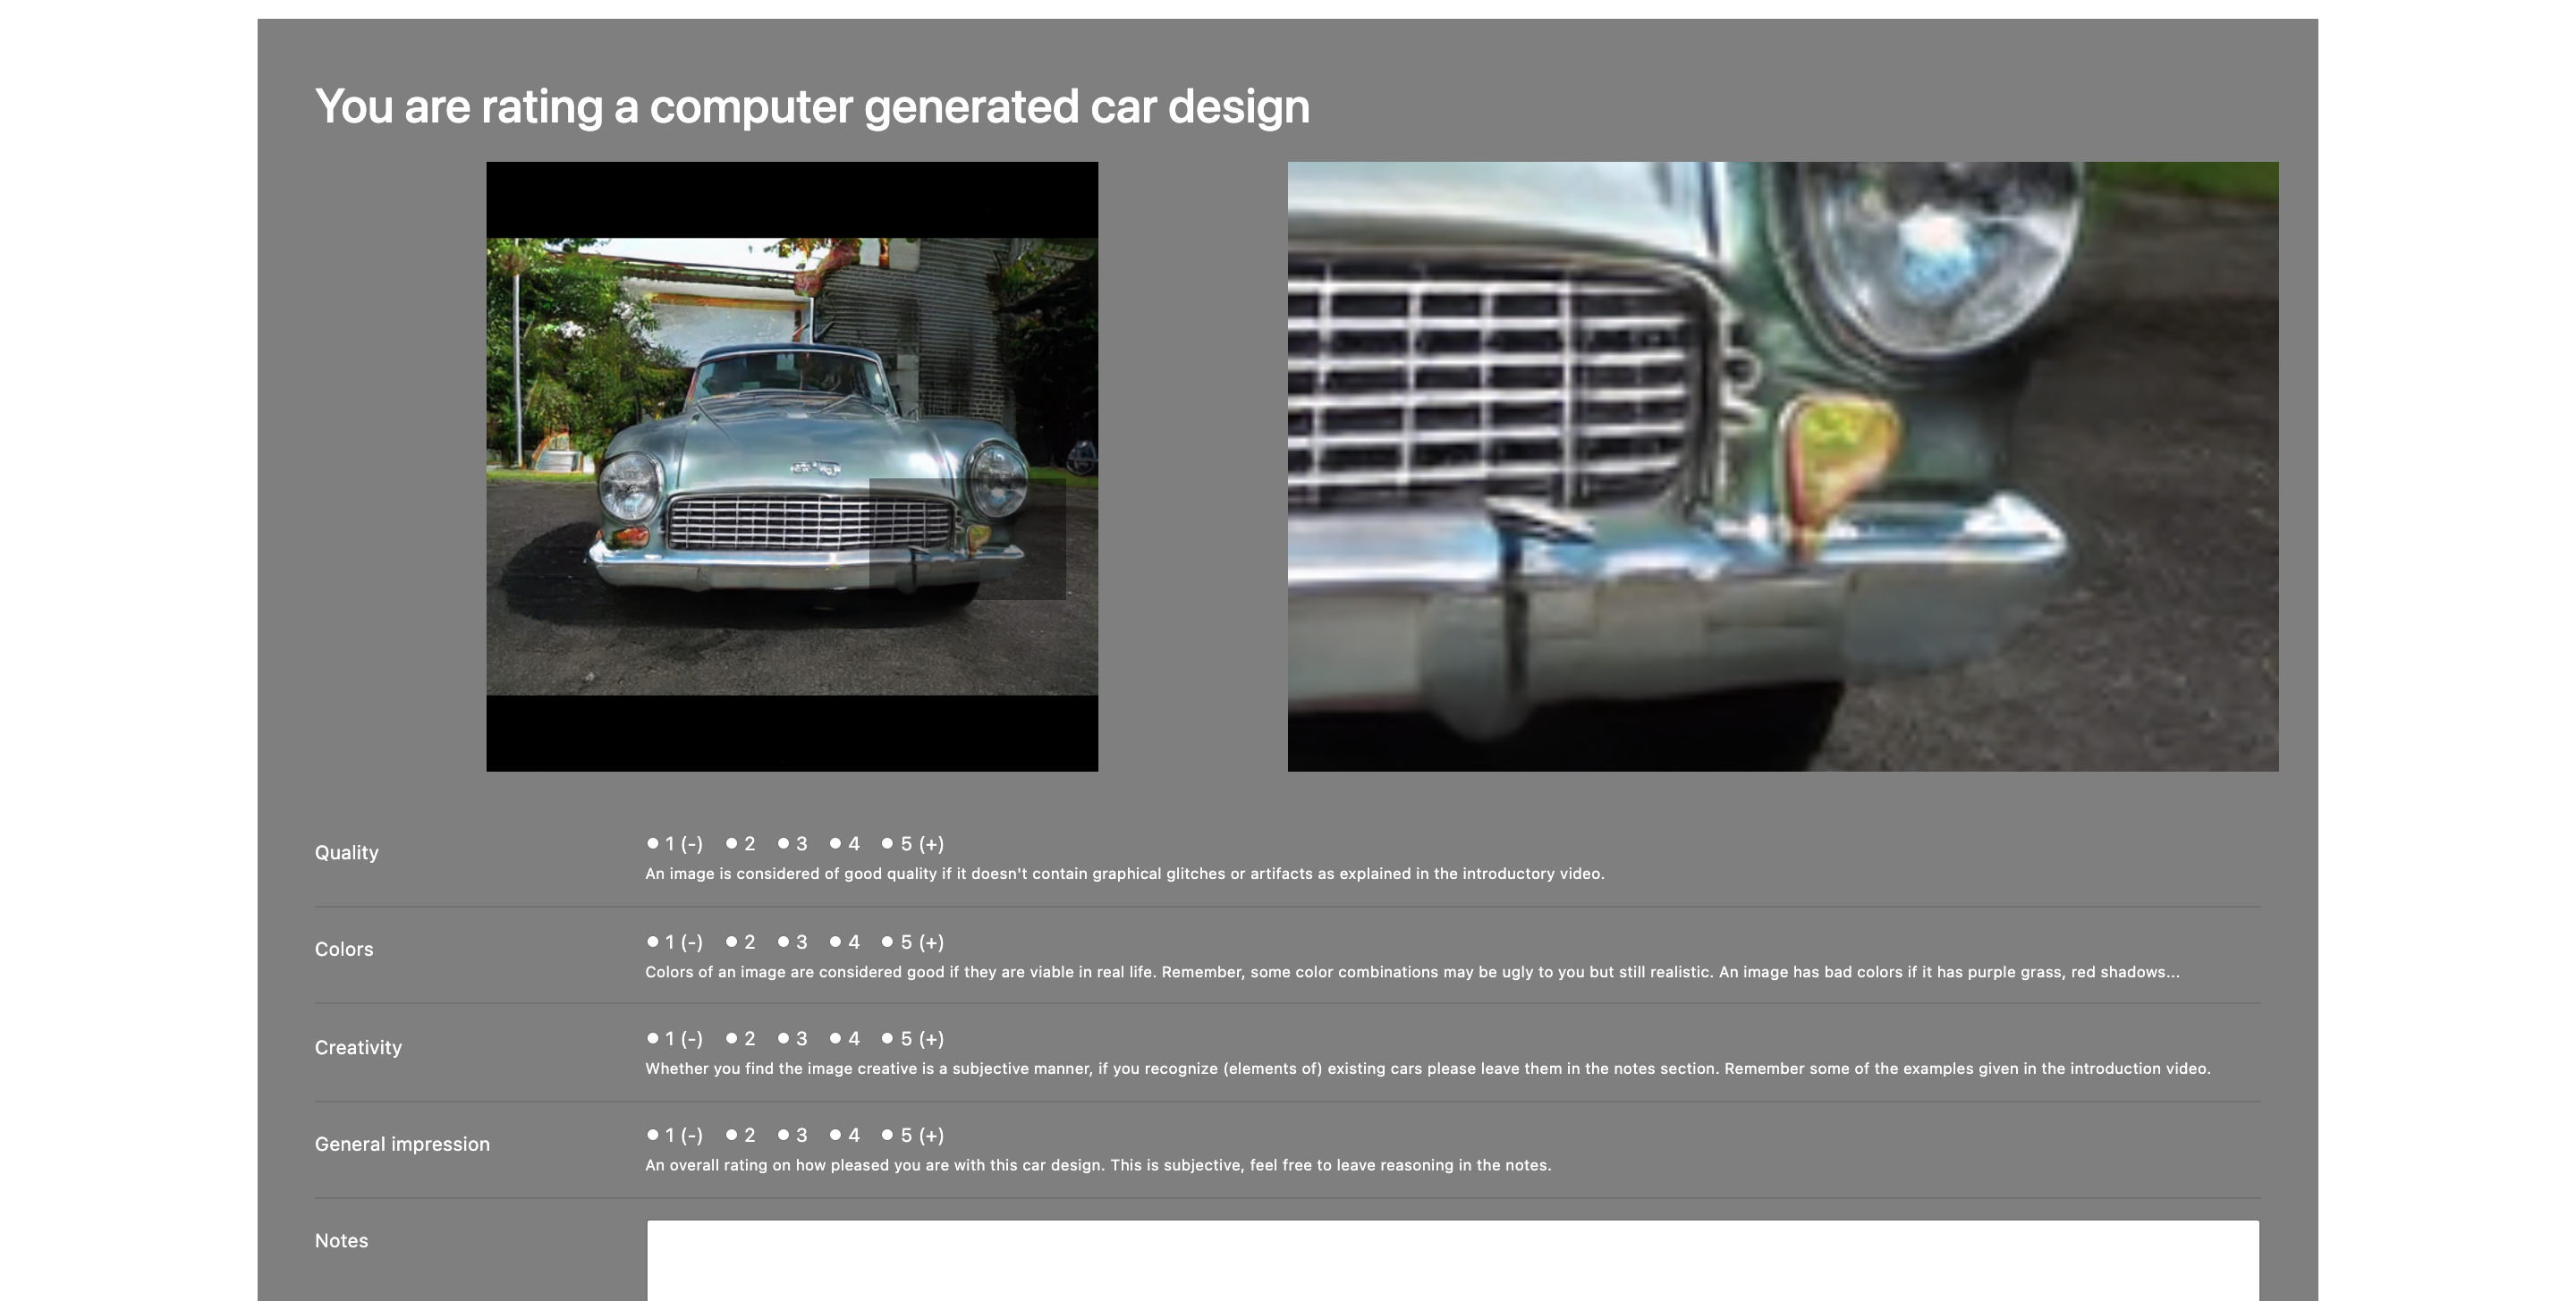
\includegraphics[width=0.85\linewidth]{images/online_survey.png}
    \captionsetup{width=0.85\linewidth}
    \captionsetup{justification=centering}
    \caption{Screenshot of the custom made online survey tool.}
    \label{fig:eval_tool}
\end{figure}